\documentclass[a4paper,11pt]{article}
\usepackage{graphicx}
\begin{document}

\bf{Results considering median:}\\

\begin{tabular}{cc}
	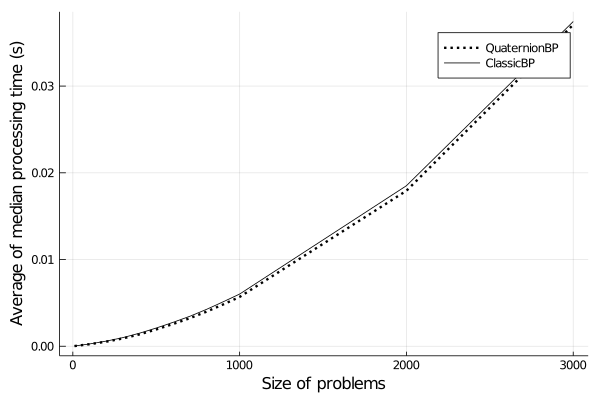
\includegraphics[width=0.5\textwidth]{perf_median_3} & 
	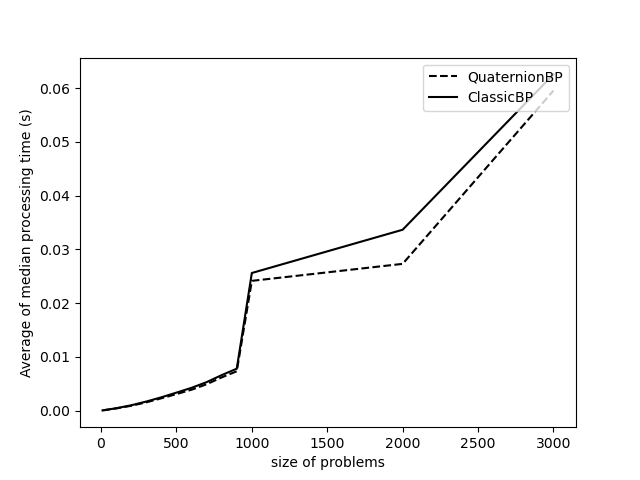
\includegraphics[width=0.5\textwidth]{perf_median_10} \\
	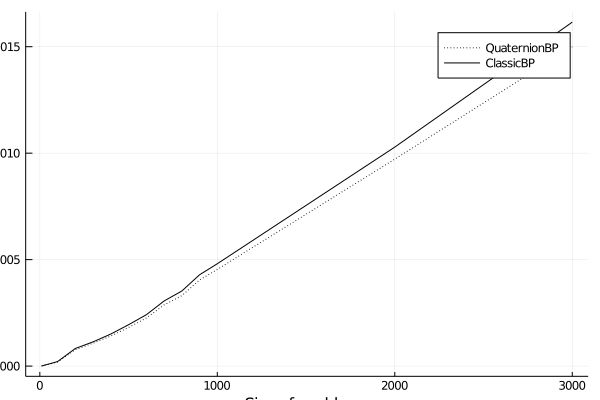
\includegraphics[width=0.5\textwidth]{perf_median_100} &
	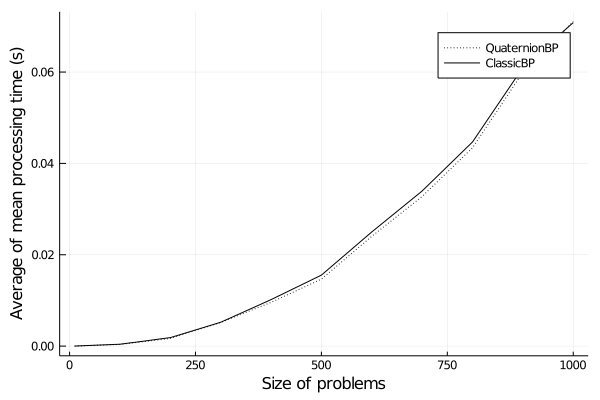
\includegraphics[width=0.5\textwidth]{perf_median_500} \\
	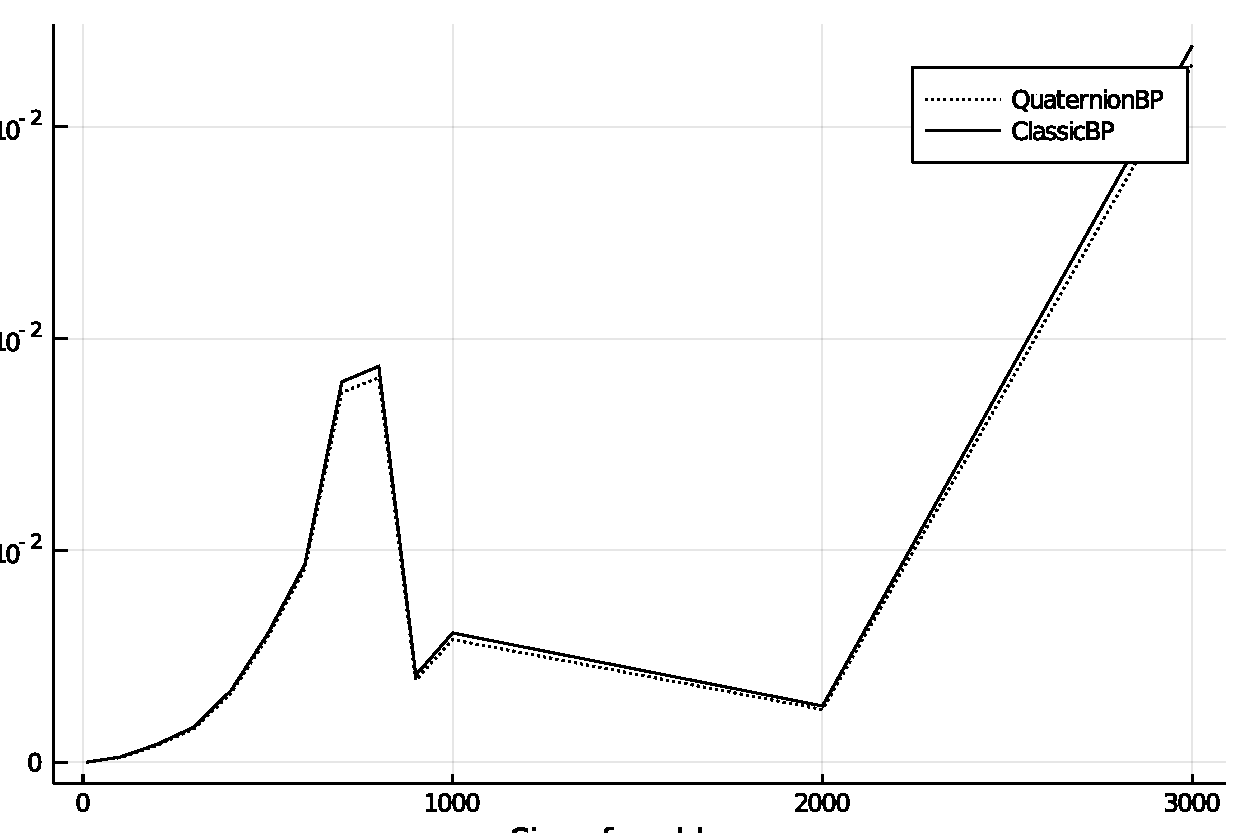
\includegraphics[width=0.5\textwidth]{perf_median_1000} &
\end{tabular}

\newpage

\bf{Results considering mean:}\\

\begin{tabular}{cc}
	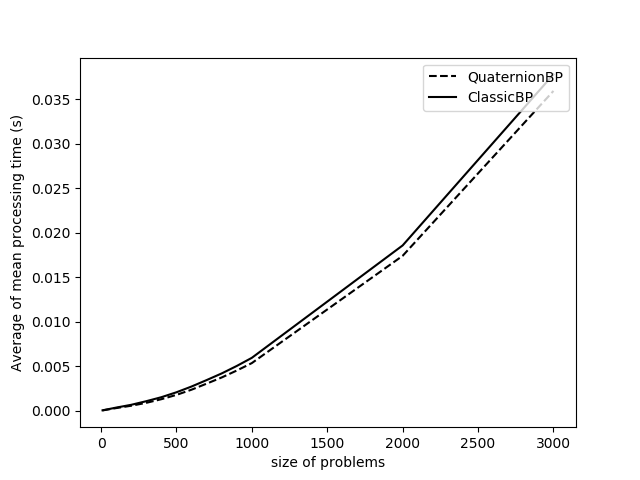
\includegraphics[width=0.5\textwidth]{perf_mean_3} & 
	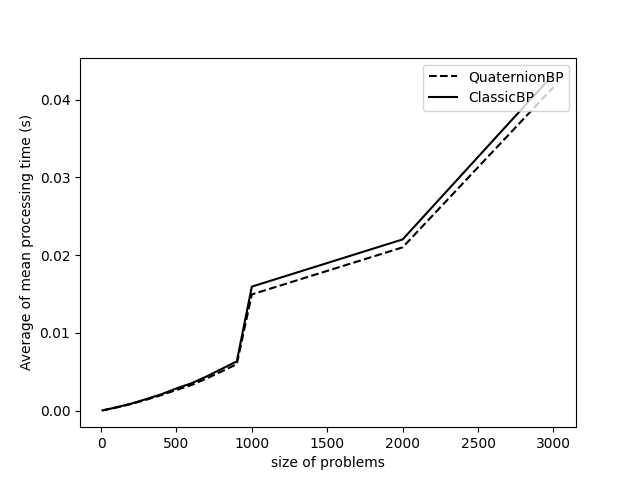
\includegraphics[width=0.5\textwidth]{perf_mean_10} \\
	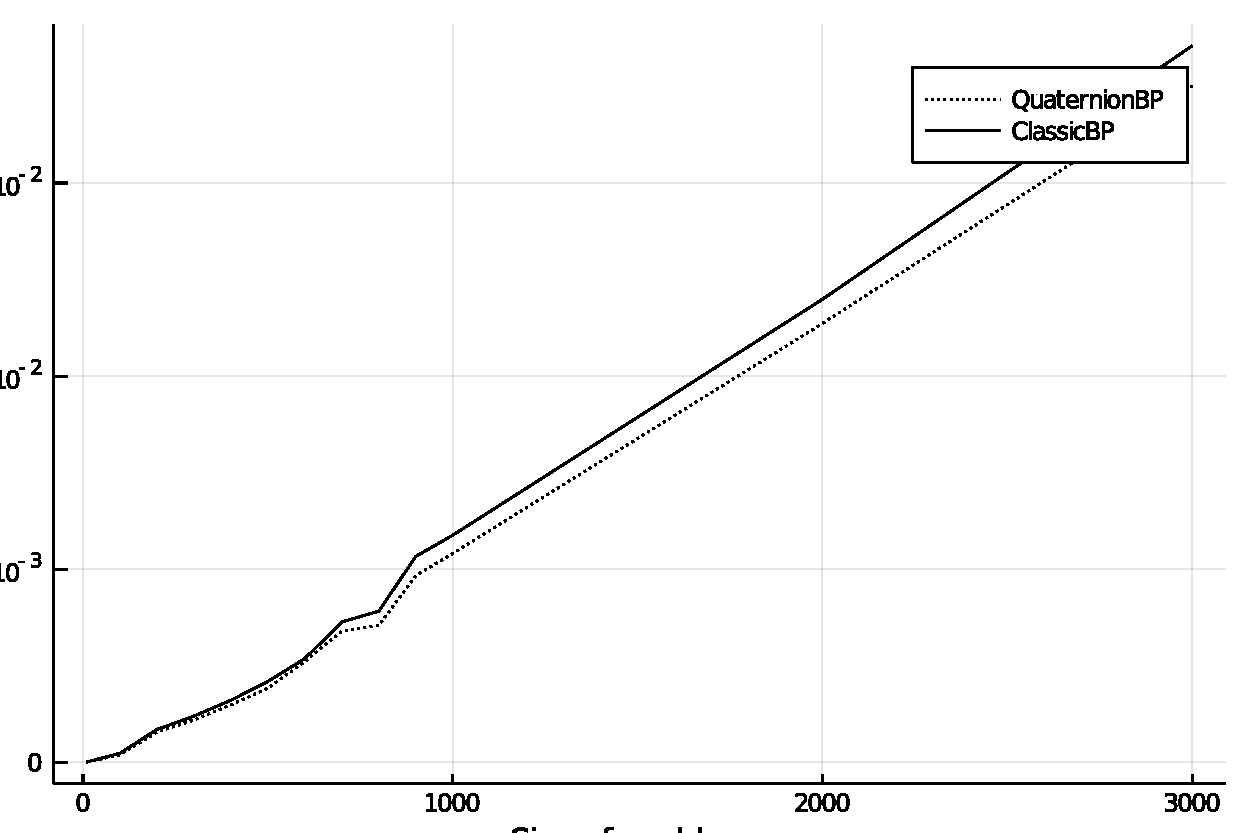
\includegraphics[width=0.5\textwidth]{perf_mean_100} &
	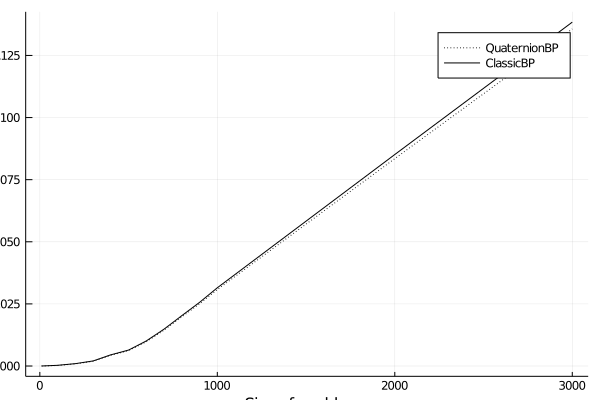
\includegraphics[width=0.5\textwidth]{perf_mean_500} \\
	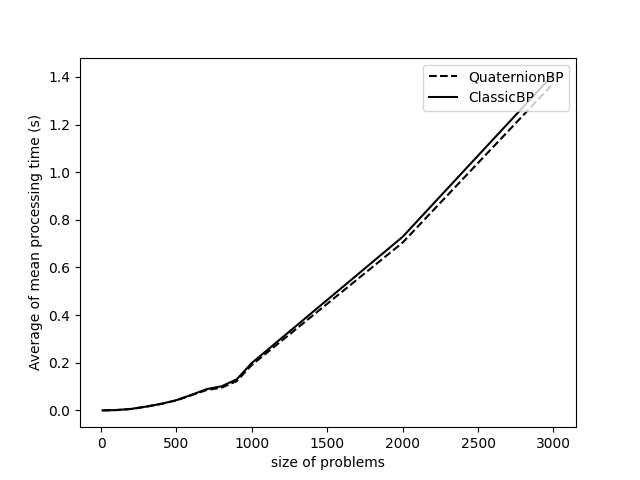
\includegraphics[width=0.5\textwidth]{perf_mean_1000} &
\end{tabular}

\newpage
\bf{Results considering minimum:}\\

\begin{tabular}{cc}
	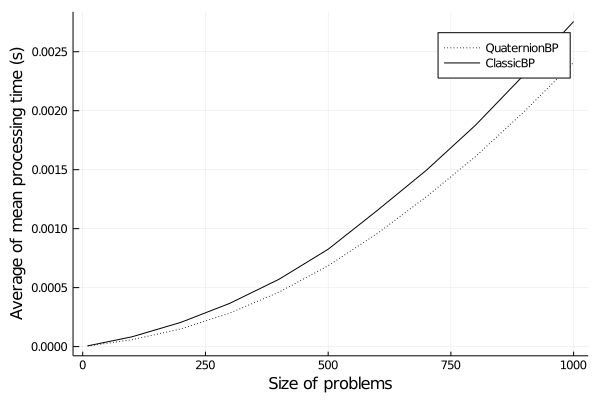
\includegraphics[width=0.5\textwidth]{perf_minimum_3} & 
	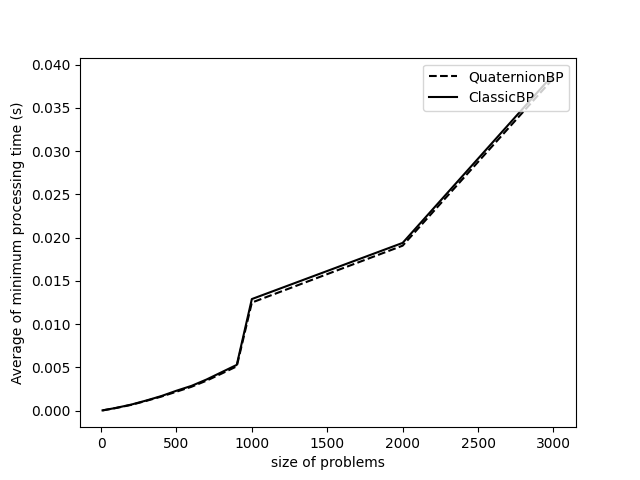
\includegraphics[width=0.5\textwidth]{perf_minimum_10} \\
	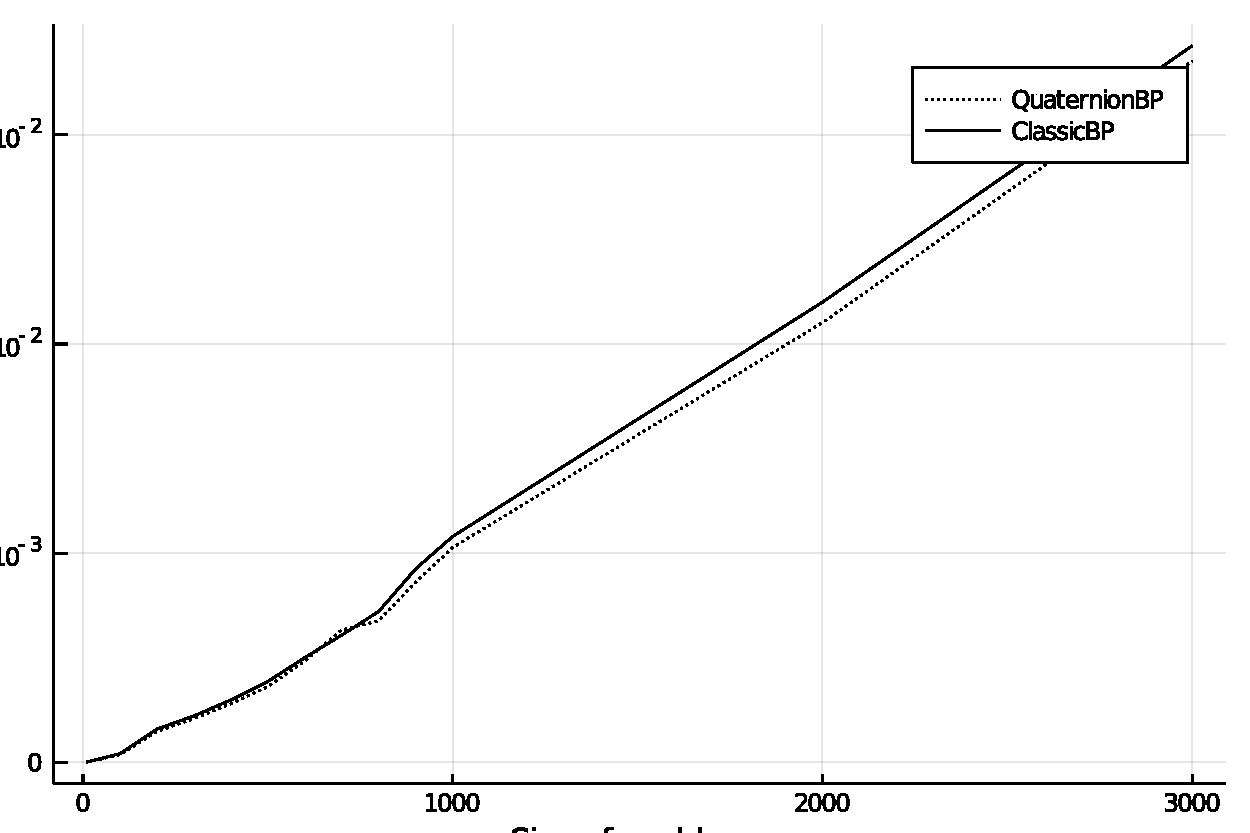
\includegraphics[width=0.5\textwidth]{perf_minimum_100} &
	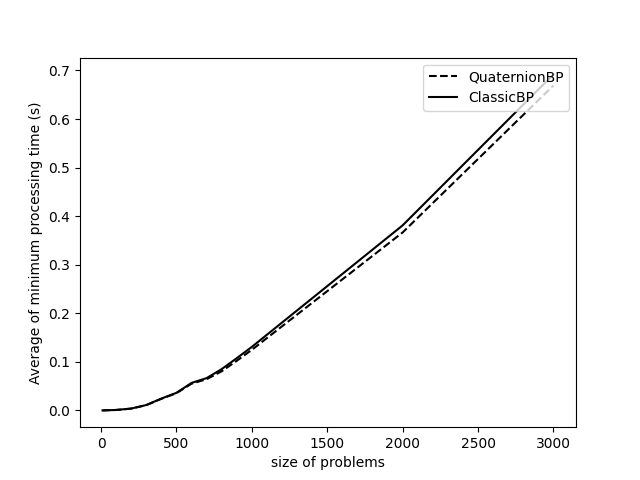
\includegraphics[width=0.5\textwidth]{perf_minimum_500} \\
	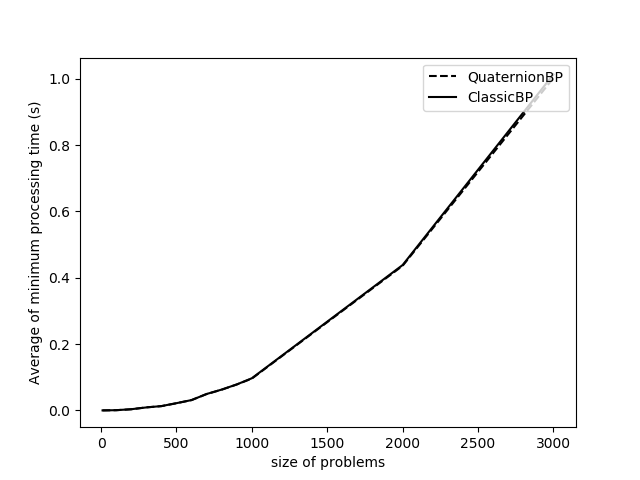
\includegraphics[width=0.5\textwidth]{perf_minimum_1000} &
\end{tabular}

\newpage
\bf{Results considering maximum:}\\

\begin{tabular}{cc}
	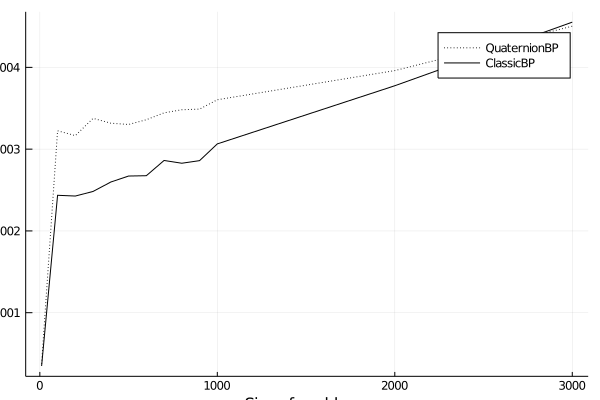
\includegraphics[width=0.5\textwidth]{perf_maximum_3} & 
	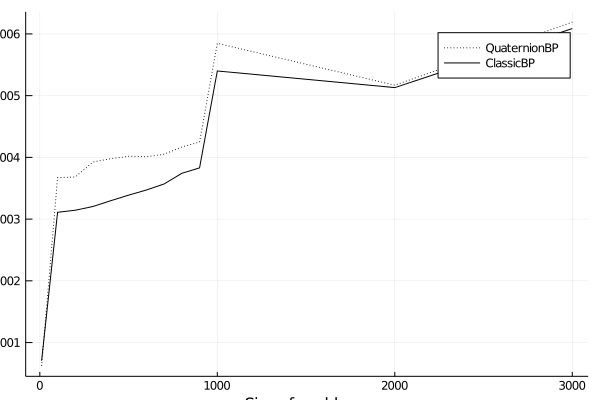
\includegraphics[width=0.5\textwidth]{perf_maximum_10} \\
	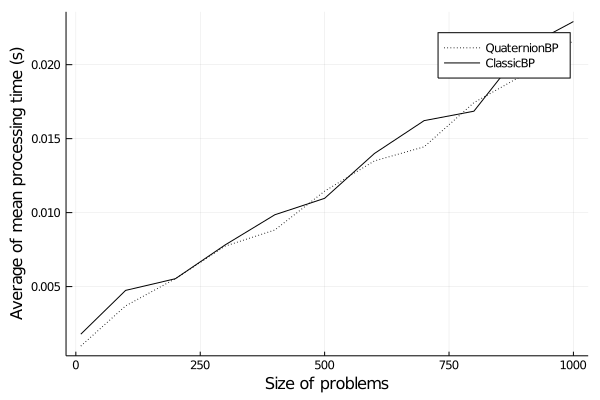
\includegraphics[width=0.5\textwidth]{perf_maximum_100} &
	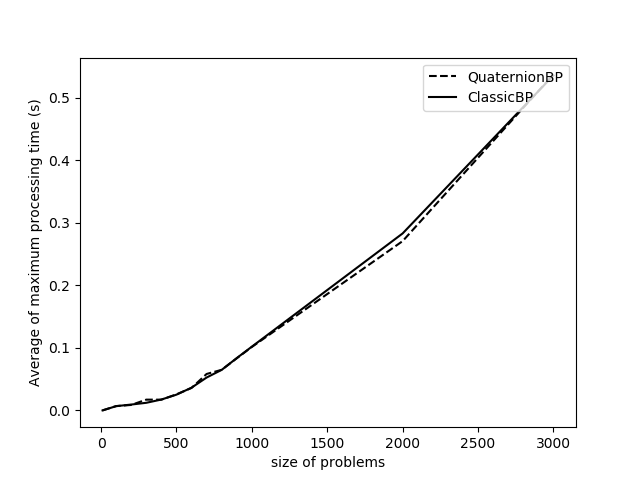
\includegraphics[width=0.5\textwidth]{perf_maximum_500} \\
	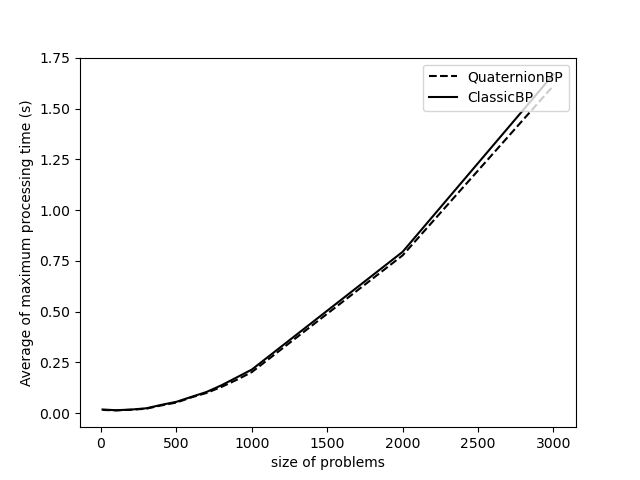
\includegraphics[width=0.5\textwidth]{perf_maximum_1000} &
\end{tabular}



\end{document}	
